Now that we selected the best combination of \emph{cache plans}, the last step is to transform the original input queries to use them. First, the execution engine should notice that the output of \emph{cache plans} will be materialized in RAM after its execution. Next, the transformation applied on the input queries is the replacement of SEs by the \emph{extraction plans} on top of the \emph{cache plans}. Remember that \emph{cache plans} are the selected covering subexpressions that covers the records for their consumers. \emph{extraction plans} are the filterings and projections applied to ensure the query output correct result.

For each input query having the SE and employing the cache plan respectively, we build an \emph{extraction plan} that compensates the cache plan such that the output of the extraction plan on top of the cache plan is equals to the output of that SE. The query rewriting in Figure \ref{fig:rewrite} is a simple example illustrating the technique. In more abstract, we build the \emph{extraction plans} by AND-ing the filtering predicates and combining the top projection columns of the SE.

\begin{figure}[!htb]
	\centering
ubstaint	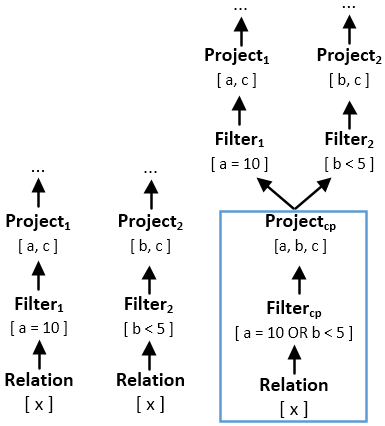
\includegraphics[scale=0.55]{figures/rewrite}
	\caption{Query rewriting example. The tree in rectangle is the cache plan}
   	\label{fig:rewrite}
\end{figure}